
%% Documentation for Parallelization of CV Algorithms using GPU
%% Authors: Andrew Kim and Joseph Angeja



\documentclass[conference]{IEEEtran}
% Some Computer Society conferences also require the compsoc mode option,
% but others use the standard conference format.
%
% If IEEEtran.cls has not been installed into the LaTeX system files,
% manually specify the path to it like:
% \documentclass[conference]{../sty/IEEEtran}





% Some very useful LaTeX packages include:
% (uncomment the ones you want to load)


% *** MISC UTILITY PACKAGES ***
%
%\usepackage{ifpdf}
% Heiko Oberdiek's ifpdf.sty is very useful if you need conditional
% compilation based on whether the output is pdf or dvi.
% usage:
% \ifpdf
%   % pdf code
% \else
%   % dvi code
% \fi
% The latest version of ifpdf.sty can be obtained from:
% http://www.ctan.org/pkg/ifpdf
% Also, note that IEEEtran.cls V1.7 and later provides a builtin
% \ifCLASSINFOpdf conditional that works the same way.
% When switching from latex to pdflatex and vice-versa, the compiler may
% have to be run twice to clear warning/error messages.






% *** CITATION PACKAGES ***
%
%\usepackage{cite}
% cite.sty was written by Donald Arseneau
% V1.6 and later of IEEEtran pre-defines the format of the cite.sty package
% \cite{} output to follow that of the IEEE. Loading the cite package will
% result in citation numbers being automatically sorted and properly
% "compressed/ranged". e.g., [1], [9], [2], [7], [5], [6] without using
% cite.sty will become [1], [2], [5]--[7], [9] using cite.sty. cite.sty's
% \cite will automatically add leading space, if needed. Use cite.sty's
% noadjust option (cite.sty V3.8 and later) if you want to turn this off
% such as if a citation ever needs to be enclosed in parenthesis.
% cite.sty is already installed on most LaTeX systems. Be sure and use
% version 5.0 (2009-03-20) and later if using hyperref.sty.
% The latest version can be obtained at:
% http://www.ctan.org/pkg/cite
% The documentation is contained in the cite.sty file itself.






% *** GRAPHICS RELATED PACKAGES ***
%
\ifCLASSINFOpdf
  \usepackage[pdftex]{graphicx}
  % declare the path(s) where your graphic files are
  \graphicspath{{.}}
  % and their extensions so you won't have to specify these with
  % every instance of \includegraphics
  \DeclareGraphicsExtensions{.pdf,.jpeg,.png}
\else
  % or other class option (dvipsone, dvipdf, if not using dvips). graphicx
  % will default to the driver specified in the system graphics.cfg if no
  % driver is specified.
  \usepackage[dvips]{graphicx}
  % declare the path(s) where your graphic files are
  \graphicspath{{../eps/}}
  % and their extensions so you won't have to specify these with
  % every instance of \includegraphics
  \DeclareGraphicsExtensions{.eps}
\fi
% graphicx was written by David Carlisle and Sebastian Rahtz. It is
% required if you want graphics, photos, etc. graphicx.sty is already
% installed on most LaTeX systems. The latest version and documentation
% can be obtained at: 
% http://www.ctan.org/pkg/graphicx
% Another good source of documentation is "Using Imported Graphics in
% LaTeX2e" by Keith Reckdahl which can be found at:
% http://www.ctan.org/pkg/epslatex
%
% latex, and pdflatex in dvi mode, support graphics in encapsulated
% postscript (.eps) format. pdflatex in pdf mode supports graphics
% in .pdf, .jpeg, .png and .mps (metapost) formats. Users should ensure
% that all non-photo figures use a vector format (.eps, .pdf, .mps) and
% not a bitmapped formats (.jpeg, .png). The IEEE frowns on bitmapped formats
% which can result in "jaggedy"/blurry rendering of lines and letters as
% well as large increases in file sizes.
%
% You can find documentation about the pdfTeX application at:
% http://www.tug.org/applications/pdftex





% *** MATH PACKAGES ***
%
%\usepackage{amsmath}
% A popular package from the American Mathematical Society that provides
% many useful and powerful commands for dealing with mathematics.
%
% Note that the amsmath package sets \interdisplaylinepenalty to 10000
% thus preventing page breaks from occurring within multiline equations. Use:
%\interdisplaylinepenalty=2500
% after loading amsmath to restore such page breaks as IEEEtran.cls normally
% does. amsmath.sty is already installed on most LaTeX systems. The latest
% version and documentation can be obtained at:
% http://www.ctan.org/pkg/amsmath





% *** SPECIALIZED LIST PACKAGES ***
%
%\usepackage{algorithmic}
% algorithmic.sty was written by Peter Williams and Rogerio Brito.
% This package provides an algorithmic environment fo describing algorithms.
% You can use the algorithmic environment in-text or within a figure
% environment to provide for a floating algorithm. Do NOT use the algorithm
% floating environment provided by algorithm.sty (by the same authors) or
% algorithm2e.sty (by Christophe Fiorio) as the IEEE does not use dedicated
% algorithm float types and packages that provide these will not provide
% correct IEEE style captions. The latest version and documentation of
% algorithmic.sty can be obtained at:
% http://www.ctan.org/pkg/algorithms
% Also of interest may be the (relatively newer and more customizable)
% algorithmicx.sty package by Szasz Janos:
% http://www.ctan.org/pkg/algorithmicx




% *** ALIGNMENT PACKAGES ***
%
%\usepackage{array}
% Frank Mittelbach's and David Carlisle's array.sty patches and improves
% the standard LaTeX2e array and tabular environments to provide better
% appearance and additional user controls. As the default LaTeX2e table
% generation code is lacking to the point of almost being broken with
% respect to the quality of the end results, all users are strongly
% advised to use an enhanced (at the very least that provided by array.sty)
% set of table tools. array.sty is already installed on most systems. The
% latest version and documentation can be obtained at:
% http://www.ctan.org/pkg/array


% IEEEtran contains the IEEEeqnarray family of commands that can be used to
% generate multiline equations as well as matrices, tables, etc., of high
% quality.




% *** SUBFIGURE PACKAGES ***
%\ifCLASSOPTIONcompsoc
%  \usepackage[caption=false,font=normalsize,labelfont=sf,textfont=sf]{subfig}
%\else
%  \usepackage[caption=false,font=footnotesize]{subfig}
%\fi
% subfig.sty, written by Steven Douglas Cochran, is the modern replacement
% for subfigure.sty, the latter of which is no longer maintained and is
% incompatible with some LaTeX packages including fixltx2e. However,
% subfig.sty requires and automatically loads Axel Sommerfeldt's caption.sty
% which will override IEEEtran.cls' handling of captions and this will result
% in non-IEEE style figure/table captions. To prevent this problem, be sure
% and invoke subfig.sty's "caption=false" package option (available since
% subfig.sty version 1.3, 2005/06/28) as this is will preserve IEEEtran.cls
% handling of captions.
% Note that the Computer Society format requires a larger sans serif font
% than the serif footnote size font used in traditional IEEE formatting
% and thus the need to invoke different subfig.sty package options depending
% on whether compsoc mode has been enabled.
%
% The latest version and documentation of subfig.sty can be obtained at:
% http://www.ctan.org/pkg/subfig




% *** FLOAT PACKAGES ***
%
%\usepackage{fixltx2e}
% fixltx2e, the successor to the earlier fix2col.sty, was written by
% Frank Mittelbach and David Carlisle. This package corrects a few problems
% in the LaTeX2e kernel, the most notable of which is that in current
% LaTeX2e releases, the ordering of single and double column floats is not
% guaranteed to be preserved. Thus, an unpatched LaTeX2e can allow a
% single column figure to be placed prior to an earlier double column
% figure.
% Be aware that LaTeX2e kernels dated 2015 and later have fixltx2e.sty's
% corrections already built into the system in which case a warning will
% be issued if an attempt is made to load fixltx2e.sty as it is no longer
% needed.
% The latest version and documentation can be found at:
% http://www.ctan.org/pkg/fixltx2e


%\usepackage{stfloats}
% stfloats.sty was written by Sigitas Tolusis. This package gives LaTeX2e
% the ability to do double column floats at the bottom of the page as well
% as the top. (e.g., "\begin{figure*}[!b]" is not normally possible in
% LaTeX2e). It also provides a command:
%\fnbelowfloat
% to enable the placement of footnotes below bottom floats (the standard
% LaTeX2e kernel puts them above bottom floats). This is an invasive package
% which rewrites many portions of the LaTeX2e float routines. It may not work
% with other packages that modify the LaTeX2e float routines. The latest
% version and documentation can be obtained at:
% http://www.ctan.org/pkg/stfloats
% Do not use the stfloats baselinefloat ability as the IEEE does not allow
% \baselineskip to stretch. Authors submitting work to the IEEE should note
% that the IEEE rarely uses double column equations and that authors should try
% to avoid such use. Do not be tempted to use the cuted.sty or midfloat.sty
% packages (also by Sigitas Tolusis) as the IEEE does not format its papers in
% such ways.
% Do not attempt to use stfloats with fixltx2e as they are incompatible.
% Instead, use Morten Hogholm'a dblfloatfix which combines the features
% of both fixltx2e and stfloats:
%
% \usepackage{dblfloatfix}
% The latest version can be found at:
% http://www.ctan.org/pkg/dblfloatfix




% *** PDF, URL AND HYPERLINK PACKAGES ***
%
%\usepackage{url}
% url.sty was written by Donald Arseneau. It provides better support for
% handling and breaking URLs. url.sty is already installed on most LaTeX
% systems. The latest version and documentation can be obtained at:
% http://www.ctan.org/pkg/url
% Basically, \url{my_url_here}.




% *** Do not adjust lengths that control margins, column widths, etc. ***
% *** Do not use packages that alter fonts (such as pslatex).         ***
% There should be no need to do such things with IEEEtran.cls V1.6 and later.
% (Unless specifically asked to do so by the journal or conference you plan
% to submit to, of course. )

% correct bad hyphenation here
\hyphenation{op-tical net-works semi-conduc-tor}
\usepackage{algorithm}
\usepackage{algorithmic}
\makeatletter 
\newcommand\fs@norules{\def\@fs@cfont{\bfseries}\let\@fs@capt\floatc@ruled
	\def\@fs@pre{}%
	\def\@fs@post{}%
	\def\@fs@mid{\kern3pt}%
	\let\@fs@iftopcapt\iftrue}
\makeatother
\floatstyle{norules}
\restylefloat{algorithm}

\begin{document}
%
% paper title
% Titles are generally capitalized except for words such as a, an, and, as,
% at, but, by, for, in, nor, of, on, or, the, to and up, which are usually
% not capitalized unless they are the first or last word of the title.
% Linebreaks \\ can be used within to get better formatting as desired.
% Do not put math or special symbols in the title.
\title{Parallel Implementations of Computer Vision Algorithms using a GPU}


% author names and affiliations
% use a multiple column layout for up to three different
% affiliations
\author{\IEEEauthorblockN{Andrew Kim}
\IEEEauthorblockA{Computer Science\\
California Polytechnic University, San Luis Obispo\\
Email: akim73@calpoly.edu}
\and
\IEEEauthorblockN{Joseph Angeja}
\IEEEauthorblockA{Computer Science\\
California Polytechnic University, San Luis Obispo\\
Email: jangeja@calpoly.edu}}

% conference papers do not typically use \thanks and this command
% is locked out in conference mode. If really needed, such as for
% the acknowledgment of grants, issue a \IEEEoverridecommandlockouts
% after \documentclass

% for over three affiliations, or if they all won't fit within the width
% of the page, use this alternative format:
% 
%\author{\IEEEauthorblockN{Michael Shell\IEEEauthorrefmark{1},
%Homer Simpson\IEEEauthorrefmark{2},
%James Kirk\IEEEauthorrefmark{3}, 
%Montgomery Scott\IEEEauthorrefmark{3} and
%Eldon Tyrell\IEEEauthorrefmark{4}}
%\IEEEauthorblockA{\IEEEauthorrefmark{1}School of Electrical and Computer Engineering\\
%Georgia Institute of Technology,
%Atlanta, Georgia 30332--0250\\ Email: see http://www.michaelshell.org/contact.html}
%\IEEEauthorblockA{\IEEEauthorrefmark{2}Twentieth Century Fox, Springfield, USA\\
%Email: homer@thesimpsons.com}
%\IEEEauthorblockA{\IEEEauthorrefmark{3}Starfleet Academy, San Francisco, California 96678-2391\\
%Telephone: (800) 555--1212, Fax: (888) 555--1212}
%\IEEEauthorblockA{\IEEEauthorrefmark{4}Tyrell Inc., 123 Replicant Street, Los Angeles, California 90210--4321}}




% use for special paper notices
%\IEEEspecialpapernotice{(Invited Paper)}




% make the title area
\maketitle

% As a general rule, do not put math, special symbols or citations
% in the abstract
\begin{abstract}
The amount of performance increase seen in Central Processing Units (CPUs) 
seems to be plateauing within the recent years, as both speed and thermal limits are being reached.
 However, Graphics Processing Units (GPUs) have seen exponential growth
 in performance metrics within the past few years. Recent development has allowed
 GPUs to be used, not only for rendering complex and high-resolution graphics programs,
 but also for general purpose programming. This has allowed the GPU to act as a co-processor 
 to the CPU resulting in high throughput. This harmonization between the CPU and GPU
 can be used for computationally-expensive algorithms where numerous independent
 calculations must be done to determine the final result of the program. Computer vision
 is a field that has developed within recent years to make sense of data within images.
 Algorithms within this fields are computationally expensive due to the fact that every pixel
 within the image in question must be analyzed. This paper explores the affects of using a GPU
 to create parallel implementations of both simple and complex computer vision algorithms.
\end{abstract}

% no keywords




% For peer review papers, you can put extra information on the cover
% page as needed:
% \ifCLASSOPTIONpeerreview
% \begin{center} \bfseries EDICS Category: 3-BBND \end{center}
% \fi
%
% For peerreview papers, this IEEEtran command inserts a page break and
% creates the second title. It will be ignored for other modes.
\IEEEpeerreviewmaketitle

\section{Introduction}
% no \IEEEPARstart
The Graphics Processing Unit (GPU) was originally designed to render images and videos
that the CPU would have trouble performing linearly. Computer vision, a field that has been
of great interest of recent years, aims to solve the inverse problem of graphics processing.
The goal of graphics processing is to render images from scenes. The GPU is used to 
calculate and update pixel values of an image faster than the CPU. However, a computer 
vision application tries to understand scenes from an image by analyzing the different pixel
values and recognizing patterns generated by those values. Computer vision is heavily being 
utilized within various different industries. Cell phones use it to identify the user's face for security purposes. 
Photo storage applications such as Google Photos 
also utilize computer vision to identify people in images and automatically group photos based
on the people in them or the surroundings identified in the images. However, as datasets for 
computer vision applications are continuously increasing in size, the amount of time 
to execute these programs linearly on the CPU is also increasing. The computationally-expensive
aspect of some of the algorithms in computer vision can take advantage of the parallel processing
that GPUs offer. 

Some of the more simple operations in computer vision include various types of thresholding.
Thresholding is the simplest form of image segmentation where pixels are turned black or white
based on some comparison defined by the user. The basic form of thresholding turns a pixel white
if the pixel value is greater than that of a defined constant, or black if it is less. This is done by comparing
the value of every pixel within the image with the defined constant value. There are various types of thresholding
that are used for different circumstances including binary thresholding ,adapative thresholding, RGB thresholding, etc.
These operations are not as computationally expensive as more complex algorithms, but can still be parallelized.

More complex operations in computer vision are clustering and classification algorithms. Classification
is an important data mining technique whereby a model is trained using a data set with class labels and is 
used to predict the class label of an unknown object \cite{GPUKNN1}. One of the more widely used classification algorithms
is k-nearest neighbors (kNN) \cite{kNN}. kNN is used in computer vision algorithms to classify pixels as part of 
different objects. This is done by calculating the distance between every pixel in the input image and every pixel in a training set
and using the k pixels with the shortest distances to classify the pixel in question. However, this algorithm is computationally expensive,
especially for high-resolution images and large training sets.

In this paper, we explore how performance in both simple and complex computer vision algorithms can be improved using a GPU. We implement
binary thresholding, RGB thresholding, and k-nearest neighbor algorithms and evaluate execution performance on a set of strawberry images. 
The OpenCV library is used for basic computer vision functionality such as reading in images to a matrix object. 
However, none of the OpenCV algorithms are used for benchmarking and analysis.
The OpenCL library is used for GPU programming and running the parallel components of the algorithms. 

The rest of this paper will proceed as follows. Sections II and III 
contain detailed explanations on how the thresholding and kNN algorithms work respectively and how they would run on the CPU.
In Section IV we present our parallel algorithms for each of the algorithms. Our experimental details and results are presented in Section V, and our work is summarized
in Section VI.

\section{Thresholding}
Thresholding is one of the simplest and most basic operations in computer vision. It is the simplest segmentation method
and is used to separate out regions of an image corresponding to objects which we want to analyze.
This separation is based on the variation between the pixels of the object and the pixels of the background \cite{Thresh}. 
To further understand how this process works, consider the source image with the intensity values src(x, y). The plot
in Figure 1 depicts the threshold, which is represented by the horizontal line. The values above the line are accepted values
that are part of the image to be analyzed, while values that fall below the line are blacked out.
There are various types of thresholding, and this paper analyzes two: (1) binary and (2) RGB thresholding.
\begin{figure}[h]
\centering
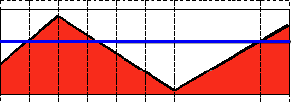
\includegraphics[width=0.3\textwidth]{ThreshDiag}
\caption{Threshold Plot Diagram}
\end{figure}

\subsection{Binary Thresholding}

Binary thresholding uses a grayscale image to segment the image into black and white pixels.
This is done by first grayscaling the input image to reduce the image to a single channel, reducing the
number values to consider from three (R, G, and B) to a single value between 0 and 255.
Once the image is converted to grayscale, each pixel value is compared to the constant threshold value.
Any of the pixels in which their color value is less than or equal to the threshold value are turned black, while
pixels with values higher than the threshold are turned white. Figure 3 shows the result of a binary threshold on the original image shown in Figure 2. 

\subsection{RGB Thresholding}
RGB thresholding is very similar to the binary threshold algorithm described above, the only difference being that all three color
channels are considered, as opposed to the one in binary threshold. Due to the fact that all three (red, green, and blue) channels are taken into account,
there is no need to grayscale the image before performing the threshold. However, the channels do need to be split and iterated through separately.
There are now three threshold values, one per channel. Each pixel is iterated through, comparing the values for the r, g, and b channels to the respective threshold
constants. If the values in all three channels for the pixel exceed their respective thresholds, then the pixel is turned white, otherwise it is turned black.
This is much more computationally expensive compared to the grayscale binary thresholding as it has to make three times the comparisons per pixel.
The results of an RGB threshold on the input image in Figure 2 is shown in Figure 4.

\newpage

\begin{figure}[h]
\centering
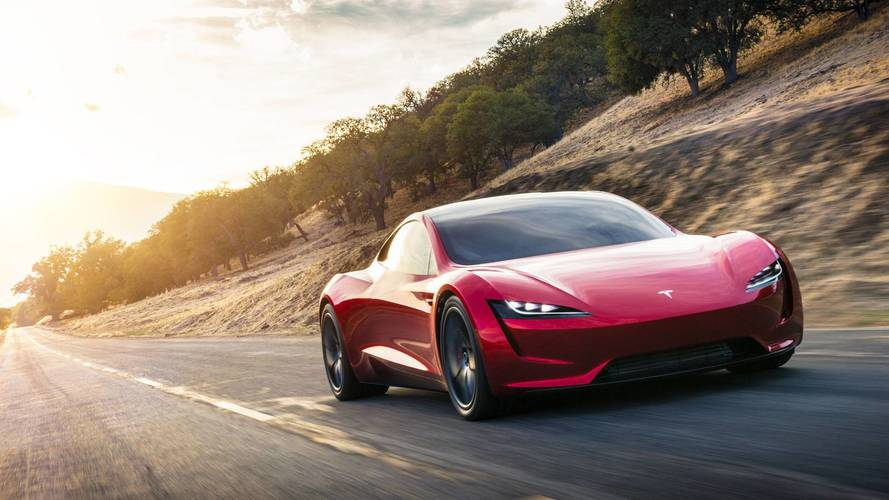
\includegraphics[width=0.3\textwidth]{thresh_in}
\caption{Original Image}
\end{figure}

\begin{figure}[h]
\centering
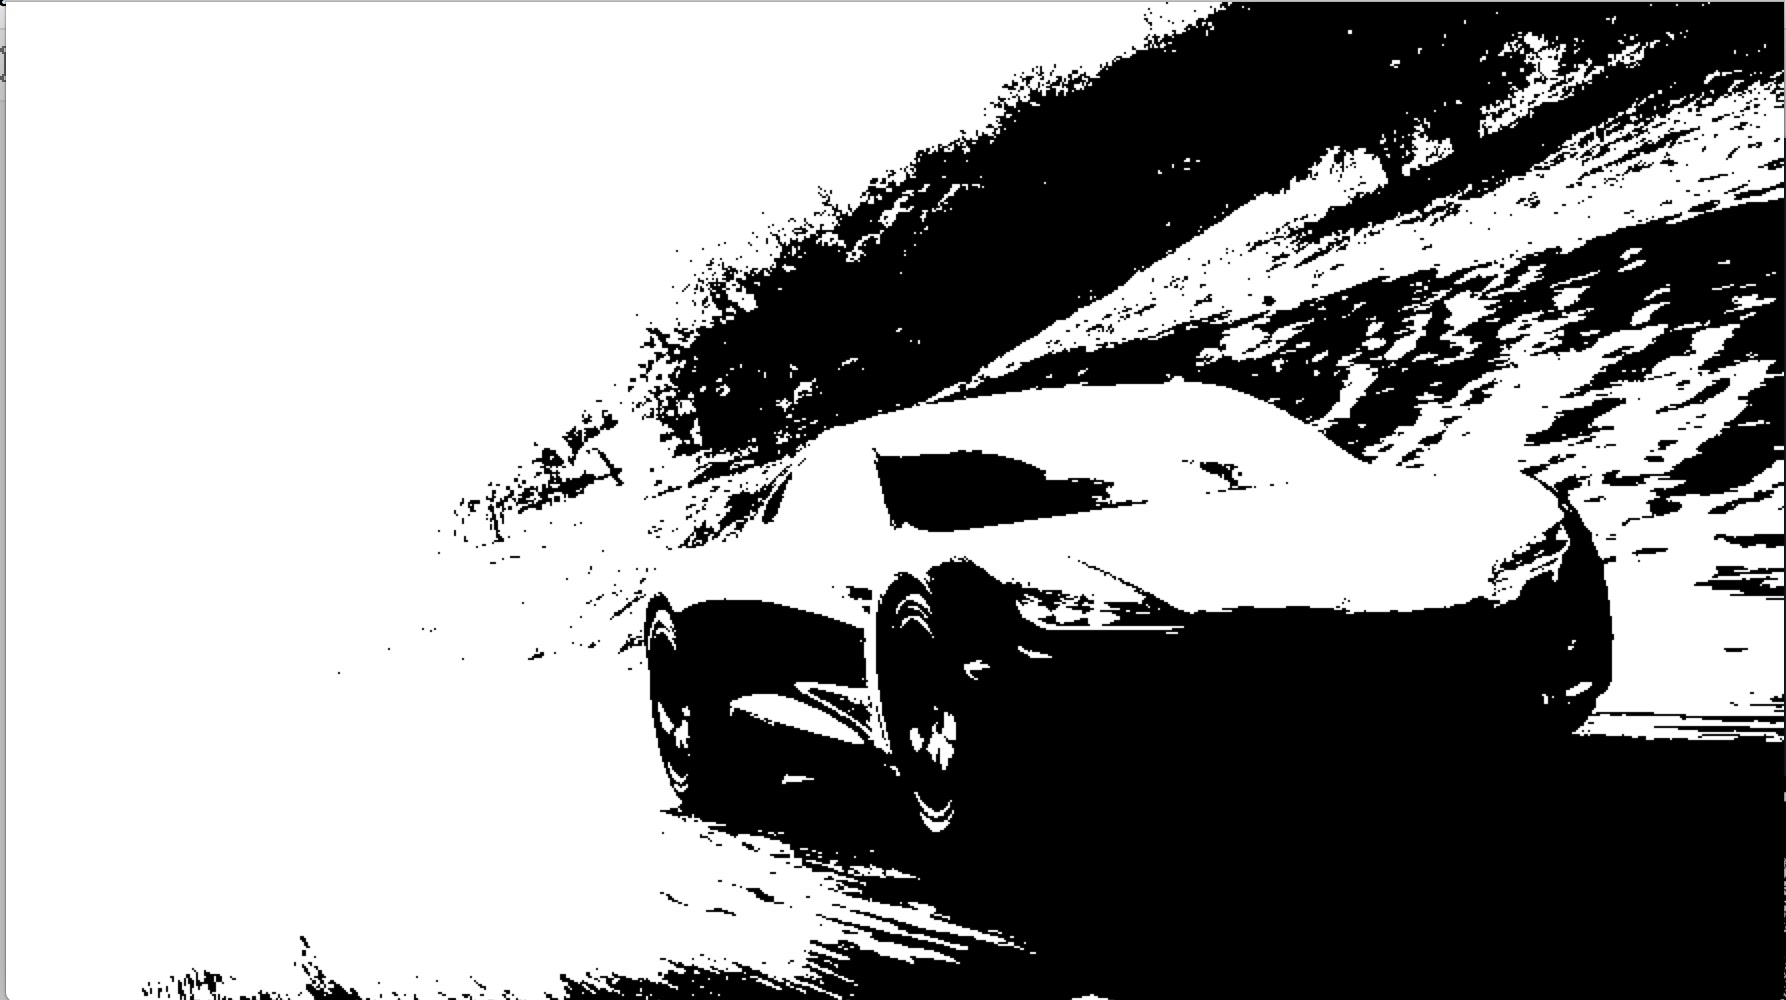
\includegraphics[width=0.3\textwidth]{thresh_bin}
\caption{Binary Threshold Results}
\end{figure}

\begin{figure}[h]
\centering
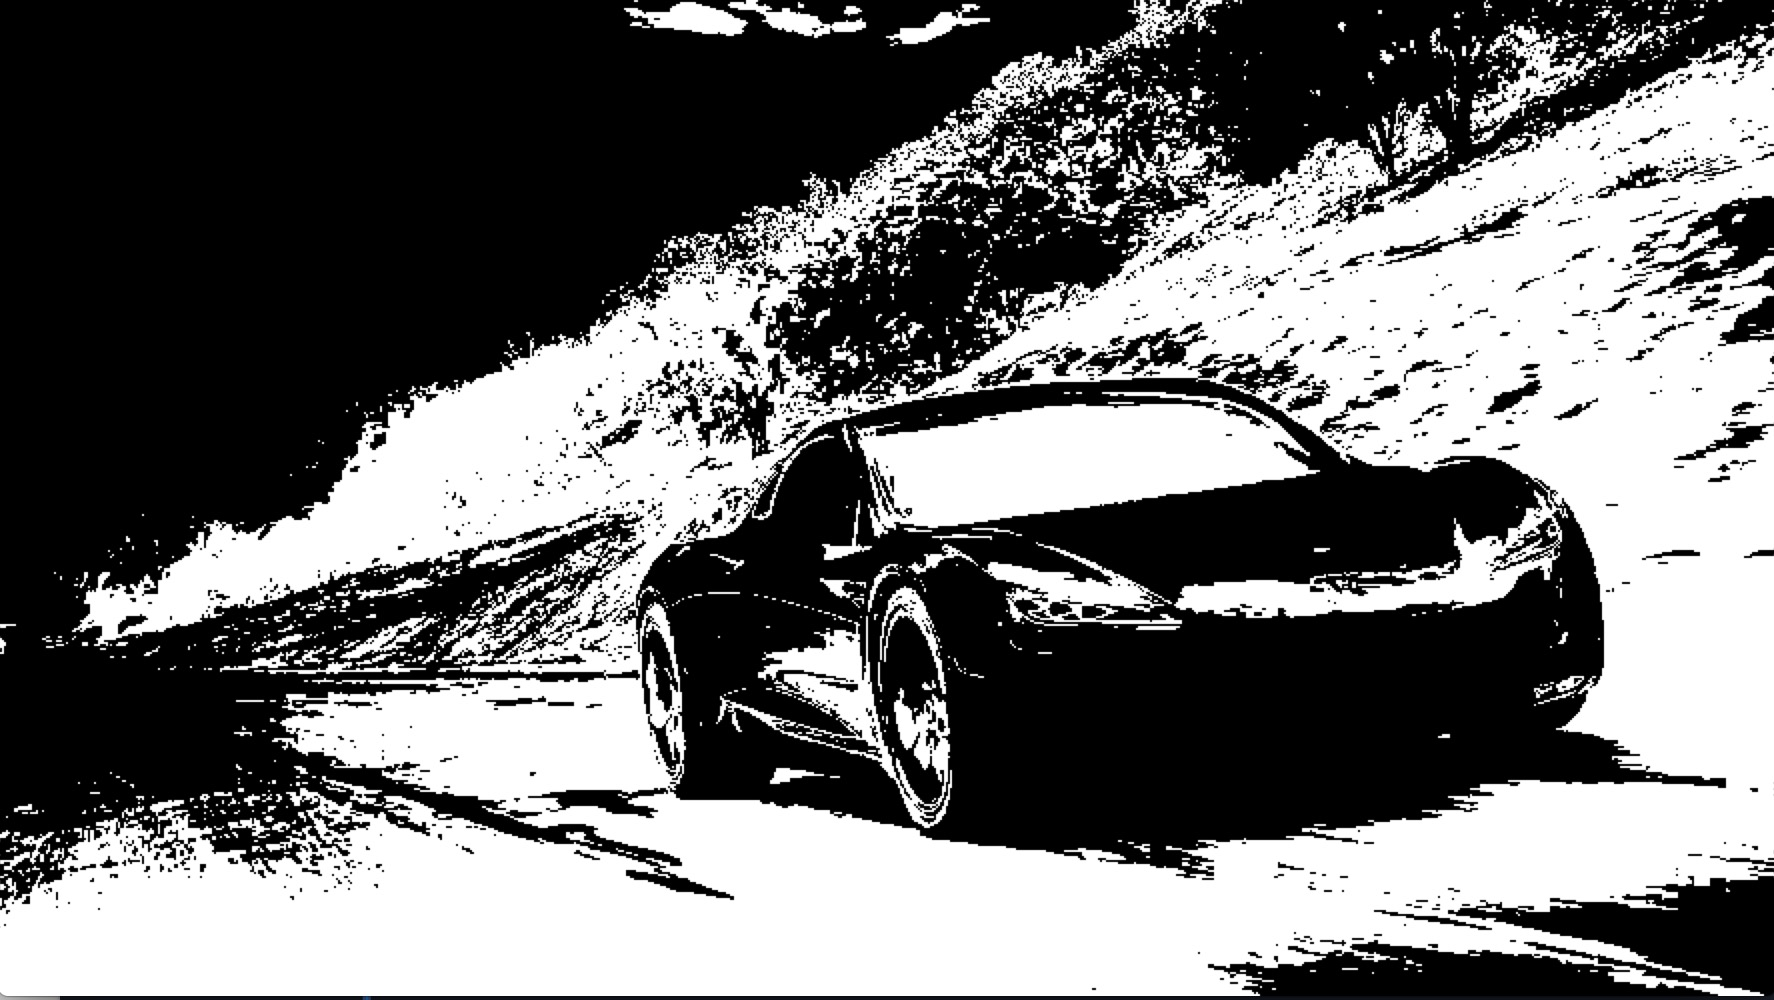
\includegraphics[width=0.3\textwidth]{thresh_rgb}
\caption{RGB Threshold Results}
\end{figure}


\section{K-Nearest Neighbors}
The kNN classification algorithm is used to predict the class of an unknown object, or pixel, by the majority of the class labels of its k nearest neighbors in the reference objects \cite{GPUKNN1}. We are interested in the brute force kNN algorithm, which is an exhaustive search which computes the distances between the pixel in question and every pixel in the training set \cite{GPUKNN2}. This classification method requires a training set with each data point in the training set classified into a cluster. For every pixel in a given unknown image, a comparison is done between every labeled pixel in the training set. At every comparison, a distance metric (Euclidean distance in this case) is calculated and stored. Once all comparisons are made, the pixels with the k shortest distances are chosen, and a majority vote is taken in order to determine the class prediction of the unknown pixel in question. Figure 5 shows an illustration of the kNN search problem with k = 3 using the Euclidean distance.

\begin{figure}[h]
\centering
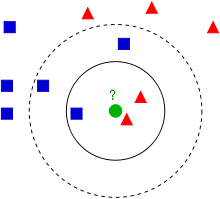
\includegraphics[width=0.3\textwidth]{knn}
\caption{RGB Threshold Results}
\end{figure}

\section{Parallel GPU Implementations}
Before the GPU is used, initialization and preparation must be done to ensure the right compute device is selected, that there is sufficient memory available, and that the correct kernel is executing on the compute units. Before executing each GPU algorithm, the following steps are taken: select the correct GPU, create a context to allow communication between the GPU and CPU, read and build the OpenCL kernel code into the CPU, initialize the command queue to issue commands to the GPU, and allocate memory on the GPU for the image that will be run through the computer vision algorithms. The computer vision algorithms reference the command queue and image buffer, so storing those are necessary. We do so by storing all relevant GPU data in a GPU data structure that we create. All of the above steps are performed within the C++ code running on the system’s CPU.

Each thread executes the same kernel code, but to divide the work, the thread \verb|id| is used. Threads are given a global \verb|id| and a local \verb|id|. The former refers to the \verb|id| of the thread in relation to all the other threads. The latter refers to the \verb|id| of the thread within a work group. Our GPU implementations did not make use of the local \verb|id|. However, the global \verb|id| played a major role in all of our kernels.

\subsection{Background}
OpenCV is an open source computer vision library, mainly for real-time applications. The library is written in C++, but it includes APIs for other languages such as Python, Java, and Matlab. It contains useful functions and algorithms for computer vision and machine learning applications including implementations of thresholding, clustering, and classification algorithms. Some of OpenCV’s implementations have the ability to take advantage of multi-core systems and GPUs \cite{OpenCL}.

OpenCV has implemented some OpenCL aware functions that require the use of a different data structure for the image, training set, etc \cite{OpenCL}. However, the OpenCL implementations are hidden behind the normal OpenCV functions which makes it difficult to determine if OpenCL is actually being utilized.

OpenCL is an open source platform for parallel computing for a wide range of systems. Its platform is abstracted in a way that permits the use of a variety of hardware accelerators such as Graphics Processing Units (GPUs), digital signal processors (DSPs), and field-programmable gate arrays (FPGAs) \cite{Khronos}. This abstraction is done by viewing all devices on a particular system as compute devices, each of which contain a number for compute units. An OpenCL kernel is executed on multiple compute units in parallel. The division of the workload depends entirely on the programmer due to the fact that the number of threads, work groups, and how the compute device is divided is fully configurable. 

The generic workflow for an OpenCL assisted program consists of the following steps: (1) build the kernel for the compute device on the CPU, (2) initialize data structures and allocate compute device memory, (3) write data to compute device buffer, (4) start kernel on compute device and let compute units on the compute device execute the kernel in parallel, (5) read the data from the compute device’s memory back into the CPU. This generic workflow is accomplished by a set of OpenCL APIs built for C and C++. The OpenCL kernels are written in a C-like language called OpenCL C that is built upon C99. They are compiled at runtime using the above described OpenCL APIs.

\subsection{Binary Thresholding}
Our implementation of binary thresholding consists of a minimum and a maximum value that pixel values must fall between to be classified as a “1”. We choose this method as opposed to the more widely used single value binary thresholding because the number of comparisons are doubled and allows for more computations to be executed on the GPU. 

\begin{algorithm}[H]
\caption{Kernel for Binary Thresholding}
\begin{algorithmic}[1]
\renewcommand{\algorithmicrequire}{\textbf{Input:}}
\REQUIRE img, min, max, numPixels, numThreads
\FOR {$id = global.id()$ to $ numPixels$}{
\STATE pixel = image[id]
\IF {($pixel >= min$ $and$ $pixel <= max$)}
\STATE pixel = 1
\ELSE 
	\STATE pixel = 0
\ENDIF

\STATE id += numThreads
}
\ENDFOR
\end{algorithmic}
\end{algorithm}

The Algorithm 1 kernel inputs five arguments: image, min, max, number of threads, and number of pixels within the image. The number of threads and number of pixels are the most important components of the kernel. It determines how much work each thread or work item will be doing on the image. The number of pixels a single thread will compute can be determined by dividing the number of pixels in the image by the number of existing threads in the kernel. Some threads will inherently execute one more pixel than others because some threads will have to process the remainder pixels. A particular thread will determine which pixel locations it is working on by first saving the \verb|thread_id| to a variable \verb|id|. If the \verb|id| is less than the number of pixels in the image, then we want to do the work on the pixel specified by the \verb|id| and increment the \verb|id| by the number of threads. These steps are repeated until \verb|id| is greater than the number of pixels. the work done for each pixel is defined as checking if the pixel grayscale value falls within the maximum and minimum thresholds. If the pixel lies within the range, then the pixel is set to 1 (white), otherwise it is set to 0 (black). 

The CPU code performs the initialization steps and hands off the computational workload to be executed in parallel to the GPU. First, the image is written to the GPU buffer and a binary threshold kernel object is created, with the arguments set accordingly. The kernel is then enqueued to run, allowing the threads of the GPU to begin computing the values of different pixels in parallel. The CPU waits until all threads are complete to read the GPU image buffer back.

\subsection{RGB Thresholding}

Our RGB thresholding method is very similar to the binary thresholding algorithm we implemented. We use a minimum and a maximum threshold values for each component in RGB which doubles the number of comparisons as compared to the standard RGB threshold algorithm. The kernel differs from the binary threshold kernel by the number of arguments received and the extra comparisons included to account for r, g, and b values. The CPU code is the same as the binary thresholding, except for the increase in number of bytes that are written to and read from the GPU because of the extra two components in RGB.

\subsection{kNN}

The kernel code for kNN is more complex. In binary and RGB thresholding all the work is done by the GPU while the CPU acts only as the director of traffic. In kNN, the GPU’s role is not as clear. We tried multiple different methods, but only one provided accurate results. Our default training set was relatively small at around 50,000 pixels to save time on the test runs.

The first working method of kNN defined the work of a thread differently than the thresholding algorithms. In the earlier algorithms, a thread worked on one or more pixels on the test image. However, in this kNN method, a thread works on one or more pixels on the training set, with all threads working on the same test image pixel. Our training set is an array of Pixel structs that we defined which contain a distance field to store the calculation of the Euclidean distance between the training set pixel and the test image pixel in question. Because classifying pixels in parallel is desired, a single training set shared by all threads is insufficient. This is because each pixel needs to calculate the distance between itself and each training set pixel and store that distance until all the distances are calculated. Because of this, it makes sense to have a copy of the training set for each pixel within the test image, but even with a small training set as ours, it becomes quiet memory intensive to do so. We combat this by only allowing a \verb|MAX_TRAININGSETS| number of pixels to be classified in parallel. This limits the number of training set copies we need to allocate on the GPU and CPU.
\begin{algorithm}[H]
\caption{Kernel for Method 1}
\begin{algorithmic}[1]
\renewcommand{\algorithmicrequire}{\textbf{Input:}} 
\REQUIRE imgPixel, trainingIndex, trainingSets[], numTrainingPixels, numThreads
\STATE train = trainingSets[index * numTrainingPixels]
\FOR {$id = global.id()$ to $ numTrainingPixels$}{
\STATE train[offset].dist = Dist(imgPixel, train[offset])
\STATE id += numThreads
}
\ENDFOR
\end{algorithmic}
\end{algorithm}

Algorithm 2, takes in five arguments: the test image pixel, the index into the array of training sets, the array of training sets, the number of pixels in one training set, and the number of threads. The threads' first step is to store the global thread id into a variable called \verb|id|. The kernel grabs one training set by using the passed in variables \verb|index| and \verb|length| of the training set. The indexing into the array is done by multiplying the index by the training set length. Similar to the thresholding algorithms, the thread executes until the \verb|id| variable is greater than the number of training set pixels. For each training set pixel, the distance to the input image pixel is calculated and the result is written back to the training set associated with that input image pixel.

As expected, the CPU plays a bigger role in this algorithm. On top of the initial setup of the binary thresholding algorithm, the CPU must create \verb|MAX_TRAININGSETS| buffer on the CPU and the GPU. Since the algorithm can only classify \verb|MAX_TRAININGSETS| test image pixels at a time, there must be some syncing of the CPU and GPU after all \verb|MAX_TRAININGSETS| test image pixels have had their distances completely calculated. This is shown in Algorithm 3.

\begin{algorithm}[H]
\caption{CPU for Method 1}
\begin{algorithmic}[1]
\renewcommand{\algorithmicrequire}{\textbf{Input:}}
\REQUIRE img, k, numThreads
\STATE trainSize = gpuTrainSets.size()
\FOR {$i = 0$ to $numPixels$}{
\STATE pixel = image[id]
\IF {($i\%$ $MAX\_TRAININGSETS == 0$)}
		\STATE trainSets[] = readBuffer(gpuTrainSets)
		\FOR {$j = 0$ to $MAX\_TRAININGSETS$} {
		\STATE sort(trainSets[j])
			\STATE class1 = SUM1(trainSets[j][0]...trainSets[j][k])
			\STATE class2 = SUM2(trainSets[j][0]...trainSets[j][k])
			\IF {{$class1 > class2$}}
				\STATE $img[j + i - MAX\_TRAININGSETS] = 0$	
			\ENDIF
		}
		\ENDFOR
\ENDIF
\STATE spawnKernel(img[i], i) % MAX_TRAININGSETS, gpuTrainSets, trainSize, numThreads)
}
\ENDFOR

\end{algorithmic}
\end{algorithm}

\section{Experiments}
After implementing binary thresholding, RGB thresholing, and kNN in both linear CPU and parallel GPU environments, each of the algorithms are compared for speed performance. As for the hardware utilized, we have an Intel Core i7 processor running at 2.7GHz as well as an AMD Radeon Pro 560 dedicated graphics card clocked at 907MHz.

\subsection{Threshold Benchmark Process}
The thresholding benchmarks are used to compare the performance between the linear (CPU) and parallel (GPU) implementations of the operations. Embedded timing callsed withing the code provide the time that it takes the entire program to run, as well as the time it takes to run the isolated thresholding functions (excludes other operations such as grayscaling). The benchmarks were run 10 times on a 1024x768 image, and the average of the results were recorded.

\subsection{kNN Benchmark Process}
To benchmark the performance of our kNN implementations, the algorithm is put to the test of identifying strawberry pixels in a given image. A training set is created using a different image of a strawberry. A mask is created and overlapped onto the image in order to classify strawberry and non-strawberry pixels for the training set. After the training process is complete, the kNN algorithm is passed in a foreign image to identify the strawberry pixels. Timing statements in the source code provided accurate time measurements of the runtime of each algorithm and critical parts of the program such as the classification process.

In order to measure how performance scales with the dataset size, the kNN algorithm is run against a combination of different sized training sets and input images. The baseline test took a 424x283 input image to classify, which was run against a 50,246 pixel count training set. We then increase the training set size to 270,800 pixels while keeping the input image size the same. This results in many more comparisons as every pixel in the input image now has to be compared to a greater amount of pixels in the training set. The final test we do is keeping the training set at the baseline value, and increasing the input image size to 1024x768. This also drastically increases the amount of computations as there are more pixels to classify. The benchmarks are intended to test in which situations does the GPU's computational throughput create the most performance increase, if any. Each of the benchmarks were run ten times with a constant value for k, and the average of the results were recorded for comparison.

\subsection{Results}

Our GPU algorithms were run with multiple different number of threads to determine the optimal number. When the test image pixel to thread ratio approached one, we saw that the GPU thresholding algorithms actually performed slightly worse than the respective CPU versions. The reason for the performance decrease as the ratio approaches one is that the overhead of creating threads to analyze each pixel is greater than having pixels analyze multiple pixels. In order to fully utilize the GPU efficiently, a thread’s creation time should be less than the time it spends doing work. We theorize that the degrading performance is due to the fact that when the ratio approaches 1, many threads are being created, but they are doing the work of only one or two pixels which takes less time than it takes to create the thread. We found the optimal pixel to thread ratio to be somewhere between 100 and 200. The tests shown below were run with a pixel to thread ratio of 100. We saw an improvement in both thresholding algorithms and this is mainly due to the GPU’s ability to analyze multiple pixels at once, whereas the CPU version must operate serially.

The GPU binary thresholding algorithm performed roughly 60\% better than the CPU algorithm when the number of threads are significantly lower than the number of pixels in the image, while the GPU RGB thresholding algorithm exhibited on average a 77\% decrease in execution time. The higher speedup with the GPU RGB algorithm compared to the GPU binary algorithm is attributed to the more comparisons being done in RGB thresholding. The graphical results are shown in Figure 6.

\begin{figure}[h]
\centering
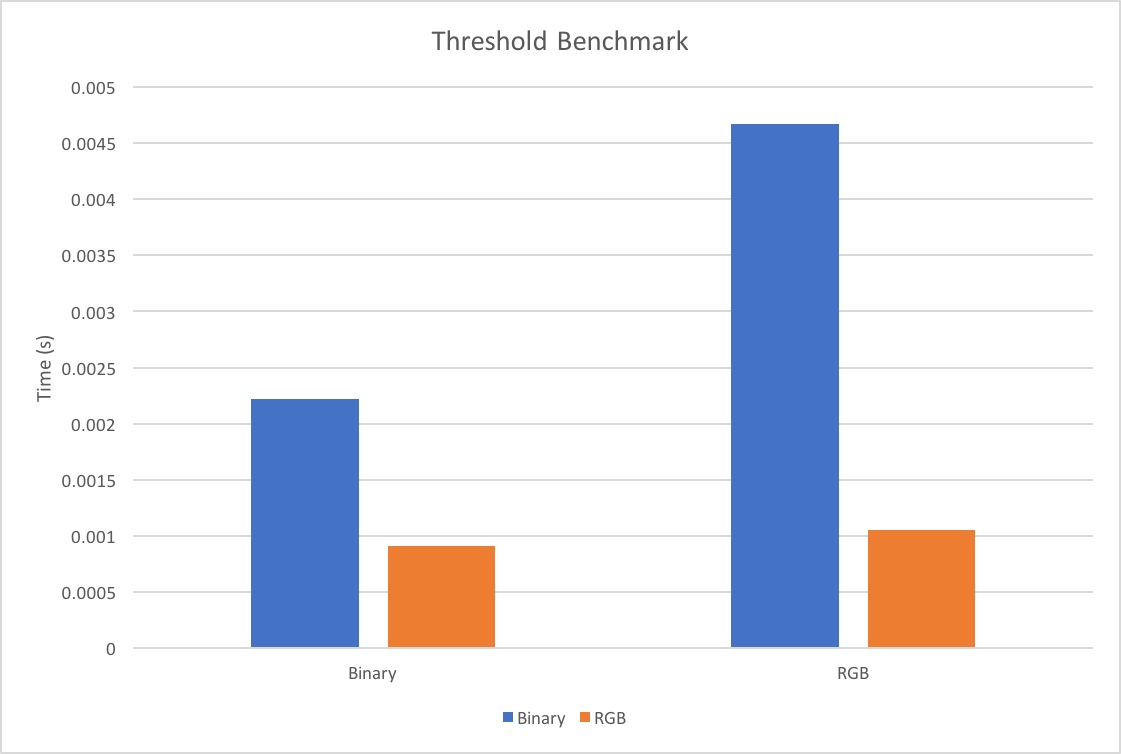
\includegraphics[width=0.5\textwidth]{threshBench}
\caption{Benchmark for Threshold Algorithms}
\end{figure}

The baseline tests show a decrease in classification time by about 10\%. The varying of the value k did not exhibit any change in the difference of overall program performance, nor did it seem to have affected the time it took to classify each pixel. We suspect this is because k plays such a small role in the actual number of computations the algorithm performs. For both k = 3 and k = 15, the algorithm still needs to calculate the distance for every pixel in the training set for every pixel in the test image. The k value only comes into play when the distance calculations are done and the distances are sorted. The algorithm then looks at the k minimum distances and runs through the voting algorithm. This small part of the kNN has magnitudes less calculations than the distance calculating and sorting. This is why there is no change in the magnitude of performance increase when changing k as shown in Figure 7.



\begin{figure}[h]
\centering
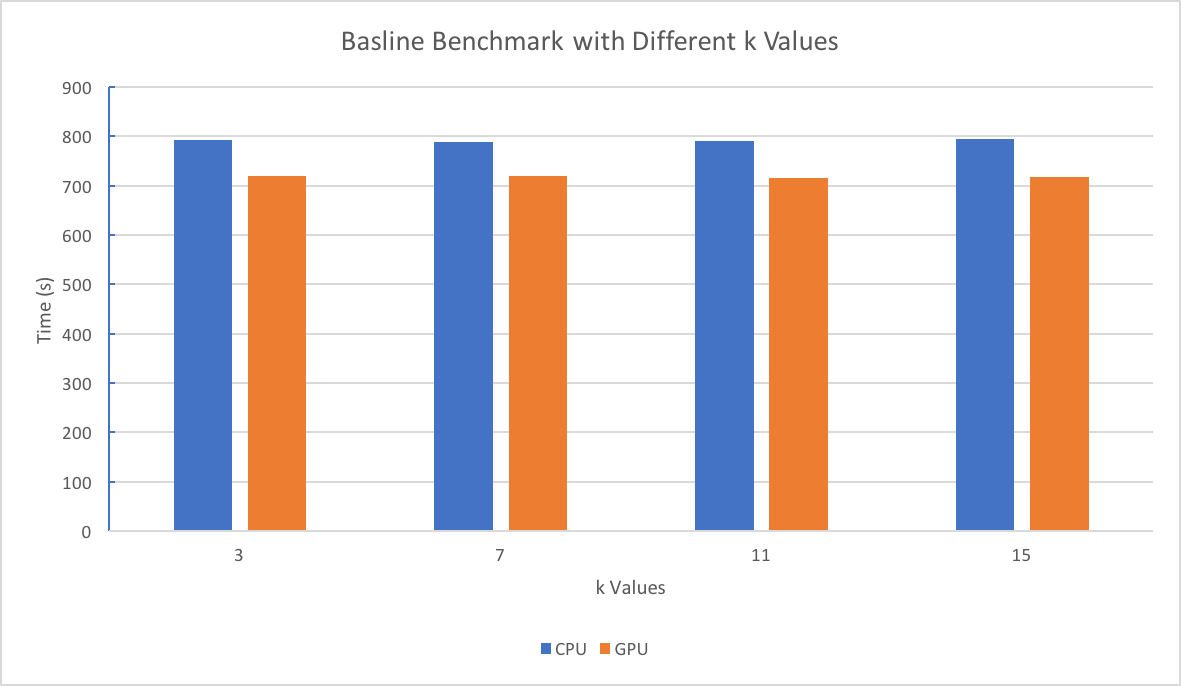
\includegraphics[width=0.5\textwidth]{diffk}
\caption{Baseline kNN with Different k Values}
\end{figure}

In the next test, we increased the training set size expecting to see a larger increase in performance due to the fact that the total number of distance calculations is over 32 billion (size of test image * size of training set) which is far more than the 6 billion pixels from the baseline test. Also, the number of test image pixels this algorithm can classify in parallel is bottlenecked by \verb|MAX_TRAININGSETS|. The training set distance calculation for one pixel is fully parallelized, so the larger the training set, the more of an increase in performance for the GPU algorithm. With this test we see about a decrease in classification time by 15\% in Figure 8.

The final test kept the same training set size and increase the test image size so we should not see the increase in performance that we saw in the second test, but we should still see something comparable to the baseline test. We saw an improvement of about 13\%.

\begin{figure}[h]
\centering
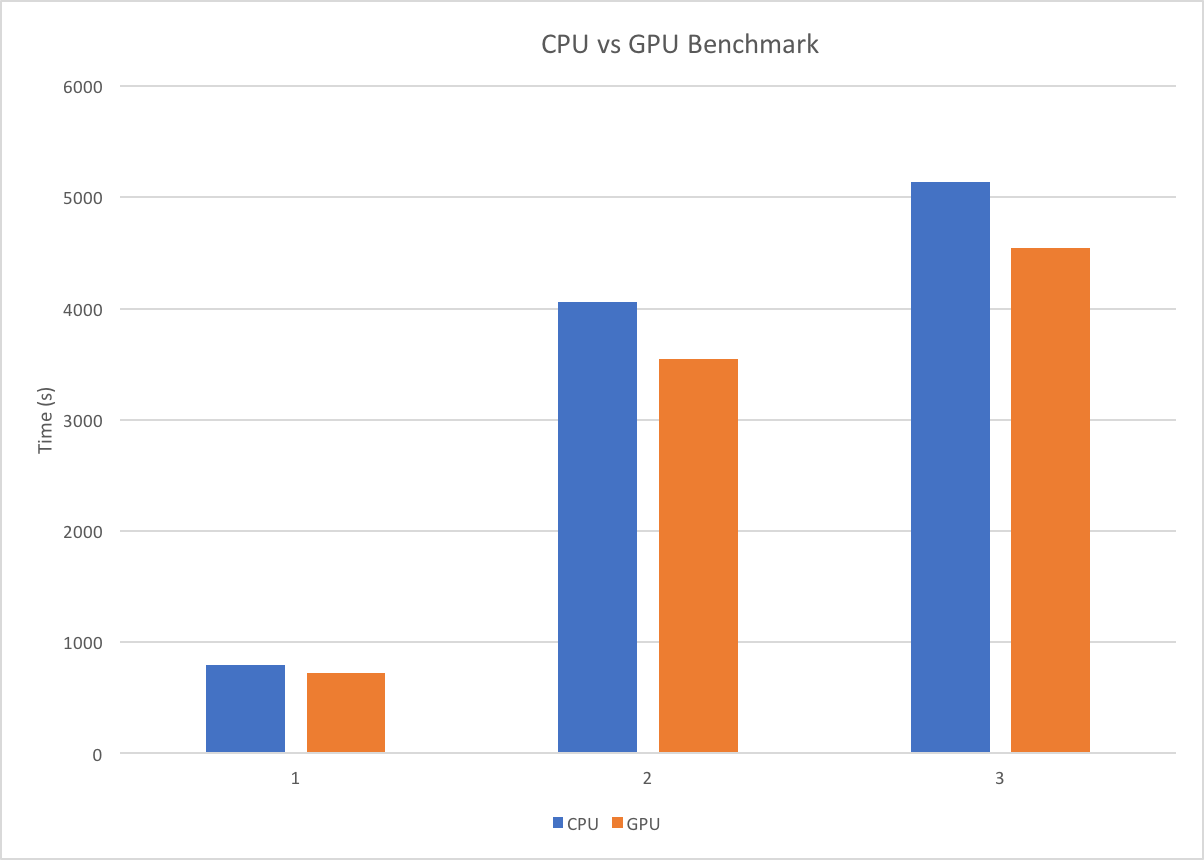
\includegraphics[width=0.5\textwidth]{bench}
\caption{Benchmark kNN with Different Image Size}
\end{figure}


% An example of a floating figure using the graphicx package.
% Note that \label must occur AFTER (or within) \caption.
% For figures, \caption should occur after the \includegraphics.
% Note that IEEEtran v1.7 and later has special internal code that
% is designed to preserve the operation of \label within \caption
% even when the captionsoff option is in effect. However, because
% of issues like this, it may be the safest practice to put all your
% \label just after \caption rather than within \caption{}.
%
% Reminder: the "draftcls" or "draftclsnofoot", not "draft", class
% option should be used if it is desired that the figures are to be
% displayed while in draft mode.
%
%\begin{figure}[!t]
%\centering
%\includegraphics[width=2.5in]{myfigure}
% where an .eps filename suffix will be assumed under latex, 
% and a .pdf suffix will be assumed for pdflatex; or what has been declared
% via \DeclareGraphicsExtensions.
%\caption{Simulation results for the network.}
%\label{fig_sim}
%\end{figure}

% Note that the IEEE typically puts floats only at the top, even when this
% results in a large percentage of a column being occupied by floats.


% An example of a double column floating figure using two subfigures.
% (The subfig.sty package must be loaded for this to work.)
% The subfigure \label commands are set within each subfloat command,
% and the \label for the overall figure must come after \caption.
% \hfil is used as a separator to get equal spacing.
% Watch out that the combined width of all the subfigures on a 
% line do not exceed the text width or a line break will occur.
%
%\begin{figure*}[!t]
%\centering
%\subfloat[Case I]{\includegraphics[width=2.5in]{box}%
%\label{fig_first_case}}
%\hfil
%\subfloat[Case II]{\includegraphics[width=2.5in]{box}%
%\label{fig_second_case}}
%\caption{Simulation results for the network.}
%\label{fig_sim}
%\end{figure*}
%
% Note that often IEEE papers with subfigures do not employ subfigure
% captions (using the optional argument to \subfloat[]), but instead will
% reference/describe all of them (a), (b), etc., within the main caption.
% Be aware that for subfig.sty to generate the (a), (b), etc., subfigure
% labels, the optional argument to \subfloat must be present. If a
% subcaption is not desired, just leave its contents blank,
% e.g., \subfloat[].


% An example of a floating table. Note that, for IEEE style tables, the
% \caption command should come BEFORE the table and, given that table
% captions serve much like titles, are usually capitalized except for words
% such as a, an, and, as, at, but, by, for, in, nor, of, on, or, the, to
% and up, which are usually not capitalized unless they are the first or
% last word of the caption. Table text will default to \footnotesize as
% the IEEE normally uses this smaller font for tables.
% The \label must come after \caption as always.
%
%\begin{table}[!t]
%% increase table row spacing, adjust to taste
%\renewcommand{\arraystretch}{1.3}
% if using array.sty, it might be a good idea to tweak the value of
% \extrarowheight as needed to properly center the text within the cells
%\caption{An Example of a Table}
%\label{table_example}
%\centering
%% Some packages, such as MDW tools, offer better commands for making tables
%% than the plain LaTeX2e tabular which is used here.
%\begin{tabular}{|c||c|}
%\hline
%One & Two\\
%\hline
%Three & Four\\
%\hline
%\end{tabular}
%\end{table}


% Note that the IEEE does not put floats in the very first column
% - or typically anywhere on the first page for that matter. Also,
% in-text middle ("here") positioning is typically not used, but it
% is allowed and encouraged for Computer Society conferences (but
% not Computer Society journals). Most IEEE journals/conferences use
% top floats exclusively. 
% Note that, LaTeX2e, unlike IEEE journals/conferences, places
% footnotes above bottom floats. This can be corrected via the
% \fnbelowfloat command of the stfloats package.




\section{Conclusion}
In this paper, we explored the affects of parallelizing simple and complex computer vision algorithms and examined how it affected performance. We implemented two different thresholding algorithms: binary and RGB, as well as the k-nearest neighbors classification algorithm for both the CPU and the GPU. In both cases we saw at least a 10\% increase in performance when run on the GPU as compared to the CPU. 

However, we believe that we could achieve more drastic results by using non-mobile computing hardware. The mobile GPU was not clocked nearly as fast as those meant for dedicated desktops or servers. The CPU in our system is very fast and efficient, and it does a fairly good job at keeping up execution speeds linearly on a single thread. This experiment shows that GPU-based parallel computing can contribute greatly to computer vision applications.
\\
\\

Source Code: https://github.com/ak2795/CSC\_515.git
\\
\\



% conference papers do not normally have an appendix


% use section* for acknowledgment
\section*{Acknowledgment}


The authors would like to thank Professor John Seng for instructing the CSC 515 Graduate Computer Architecture course.





% trigger a \newpage just before the given reference
% number - used to balance the columns on the last page
% adjust value as needed - may need to be readjusted if
% the document is modified later
%\IEEEtriggeratref{8}
% The "triggered" command can be changed if desired:
%\IEEEtriggercmd{\enlargethispage{-5in}}

% references section

% can use a bibliography generated by BibTeX as a .bbl file
% BibTeX documentation can be easily obtained at:
% http://mirror.ctan.org/biblio/bibtex/contrib/doc/
% The IEEEtran BibTeX style support page is at:
% http://www.michaelshell.org/tex/ieeetran/bibtex/
%\bibliographystyle{IEEEtran}
% argument is your BibTeX string definitions and bibliography database(s)
%\bibliography{IEEEabrv,../bib/paper}
%
% <OR> manually copy in the resultant .bbl file
% set second argument of \begin to the number of references
% (used to reserve space for the reference number labels box)
\begin{thebibliography}{1}

\bibitem{GPUKNN1}
Shenshen~Liang, Ying~Liu, Cheng~Wang, Liheng~Jian, \emph{Design and Evaluation of a Parallel K-Nearest Neighbor Algorithm on
CUDA-enabled GPU}, IEEE 2010.
  
 \bibitem{kNN}
 M. Kamber, J. Han, \emph{Data Mining: Concepts and Techniques}, 2nd Edition, Morgan Kaufmann, 2005.
  
 \bibitem{GPUKNN2}
 Vincent Garcia, E´ric Debreuve, Frank Nielsen, Michel Barlaud, \emph{K-Nearest Neighbor Search: Fast GPU-Based Implementations and Application
 to High-Dimensional Feature Matching}, 2010 IEEE 17th International Conference on Image Processing.
 
 \bibitem{Thresh}
 \emph{Basic Thresholding Operations},\\ https://docs.opencv.org/2.4/doc/tutorials/imgproc/threshold/threshold.html.
 
 \bibitem{OpenCL}
 \emph{OpenCL}, https://opencv.org/platforms/opencl.html
 
 \bibitem{OpenCV}
 \emph{OpenCV}, https://opencv.org
 
 \bibitem{Khronos}
 \emph{The open standard for parallel programming of heterogeneous systems}, https://www.khronos.org/opencl/

\end{thebibliography}




% that's all folks
\end{document}


